\documentclass{article}
\usepackage{parskip}
\usepackage{pdfpages}
\usepackage{hyperref}
\usepackage{amsmath}
\usepackage[margin=.6in]{geometry}
\begin{document}

Say we have an apple, orange, and blueberry. They each have a set of features, like color and size. So we graph size relative to color, two dimensions of features, thus the feature space is two dimensional. The feature space is usually given.

We want to create clusters where the distance between elements in the same cluster is small but the distance between clusters is big. So we have an optimization problem.

Classification problems are what we have been doing, supervised learning. Clustering is when the data is unlabeled, unsupervised.

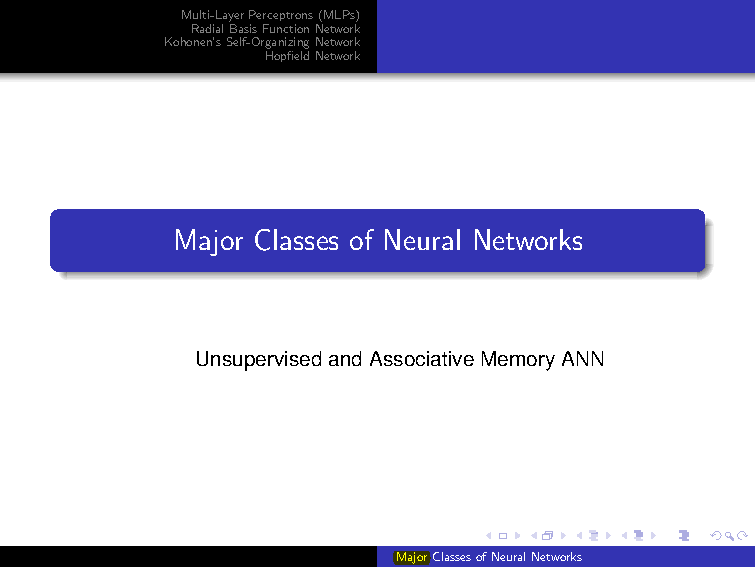
\includepdf[page=3]{slides}
You output is a series of areas clustering your input data.

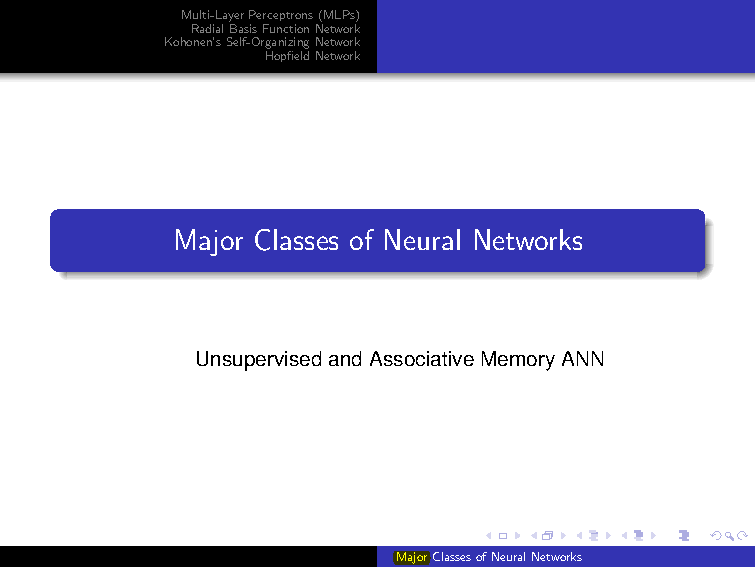
\includepdf[page=4]{slides}
Here we do not have any labels to compare against.

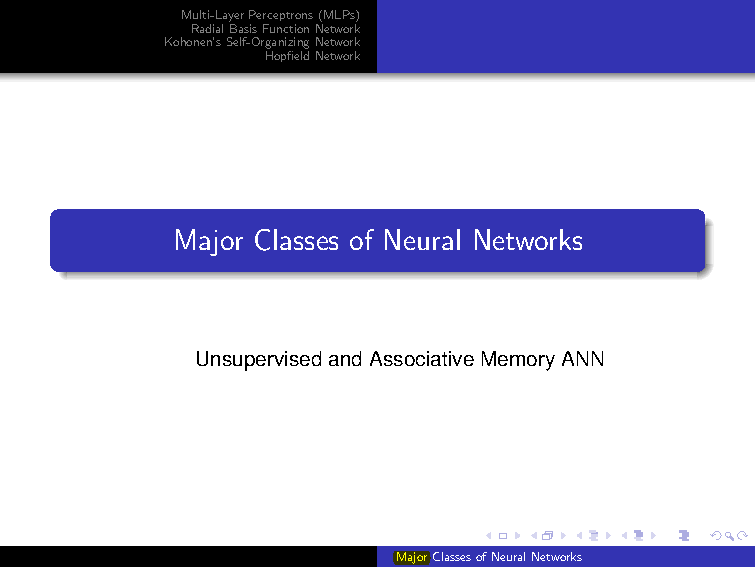
\includepdf[page=5]{slides}
The nodes distrubute themselves across the space.

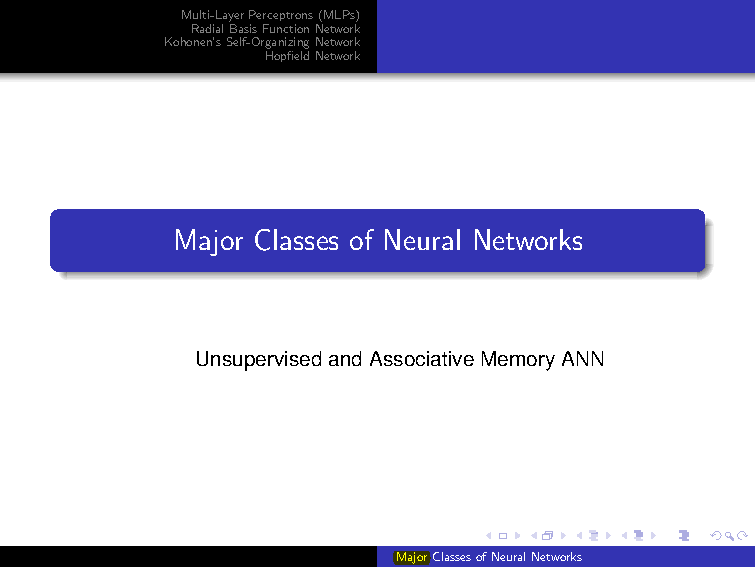
\includepdf[page=6]{slides}
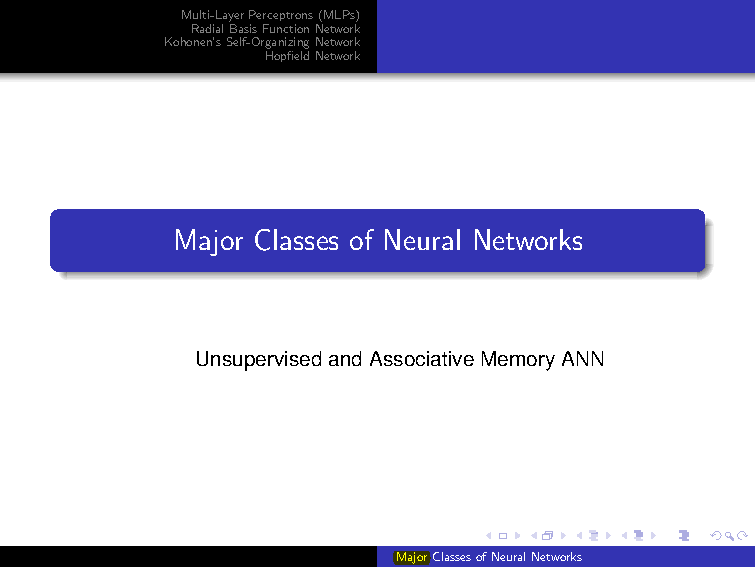
\includepdf[page=7]{slides}
 We have a input vector that we dispatch piecewise. Elements with equivalent features will occupy the same space in the output space.

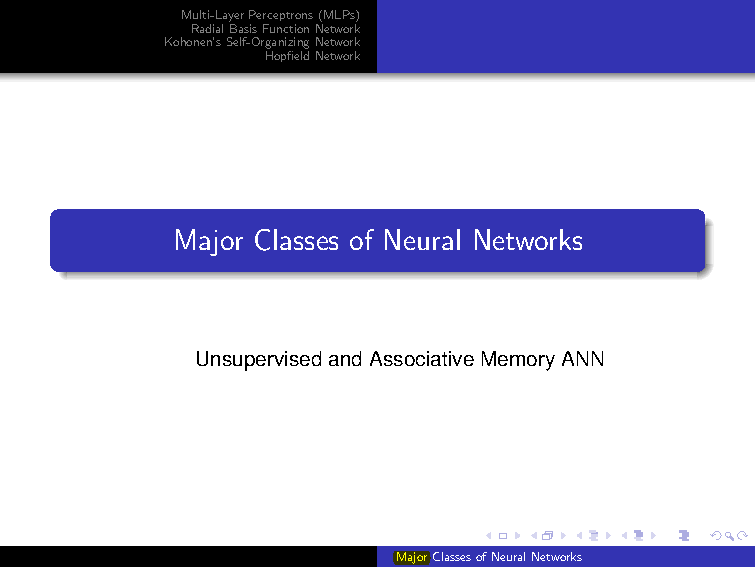
\includepdf[page=8]{slides}
We cluster the input data into smaller groups of elements with similar features. We are mapping an input space to an output space (possibly of smaller dimension).

When you dispatch a particular element there is a single winner. Suupose we have an input vector x and a weight vector w.

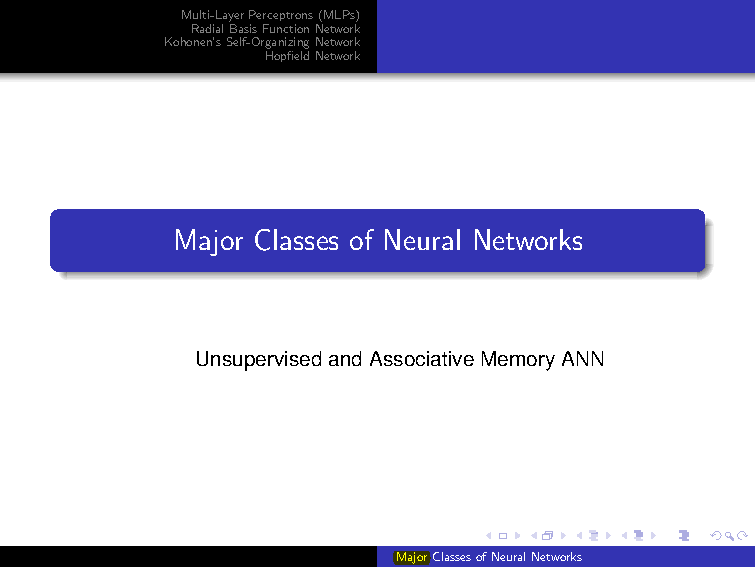
\includepdf[page=9]{slides}
NC iw the neighbors around the winning output. They are smaller winners because their feature space is close to the winner. Everytime you iterate the system the size of the neighborhood shrinks.

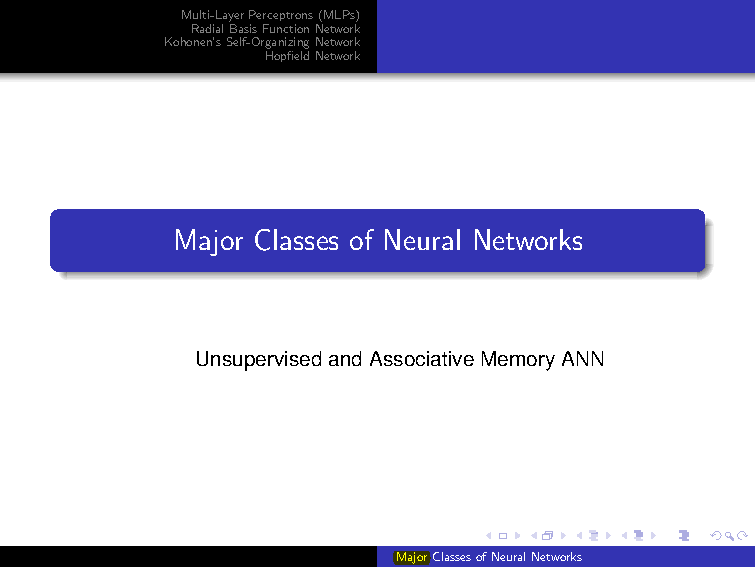
\includepdf[page=10]{slides}
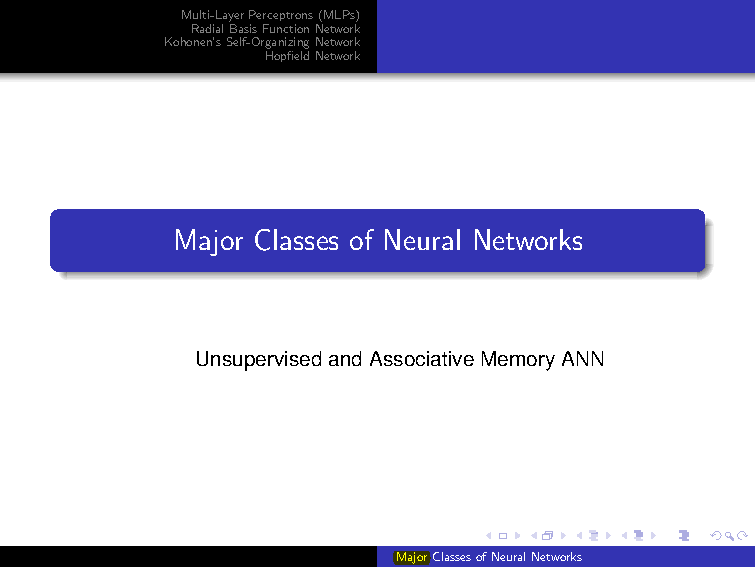
\includepdf[page=11]{slides}
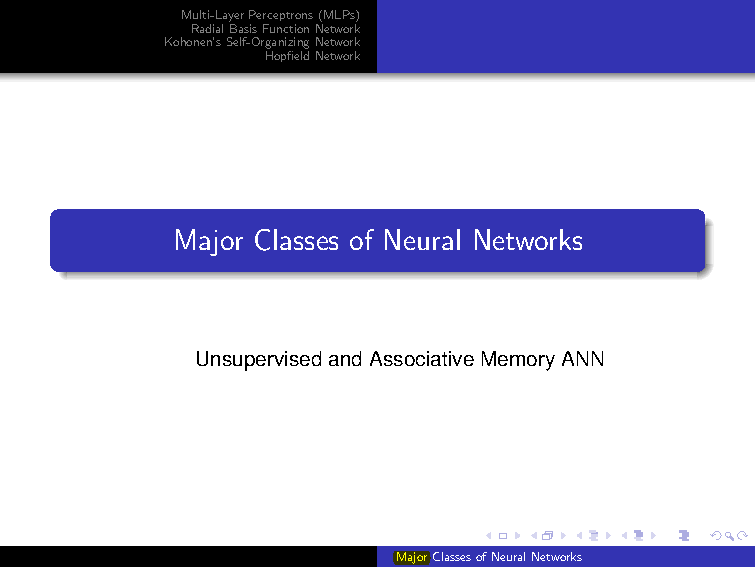
\includepdf[page=15]{slides}
Initialize all weights to small random value. Initialize the learning rate $\alpha$ to some small value for the learning rate.

Take a input patter from data set (a single element with many features)

Select the winning unit from the output space. $\omega_c$ is the weight linking the input space to output space. At start these weights are random so we start randomly.

The weights connecting the input vector to the winning node get updates (all the other weights stay the same). $\alpha(k)$ is the adaptive learning rate, it decreases as things cycle. $N_c$ is the neighborhood of the winner

We then need to update the learning rate. The rate at which it decreases is based on tunable parameters

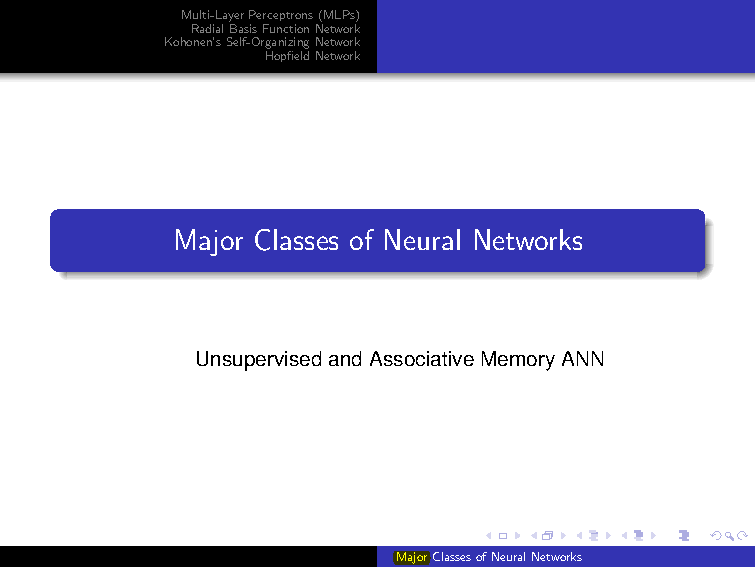
\includepdf[page=16-28]{slides}
We have three output nodes and 4 dimensional inputs.

The original learning rate is 0.3 and it decreases by multiplying it by 0.2 each time.

The feature map shows the input dimensions to output nodes with weights.

We chose an initial neighborhod size of 0, so only one winner.

Stepping through we dispatch the first input. We take the minimum

Then we update the weights based on who won.

We repeate for each input vector

Now the epoch is complete and we need to update the learning rate.

We keep repeating this cycle until all weights are steady within some threashold.


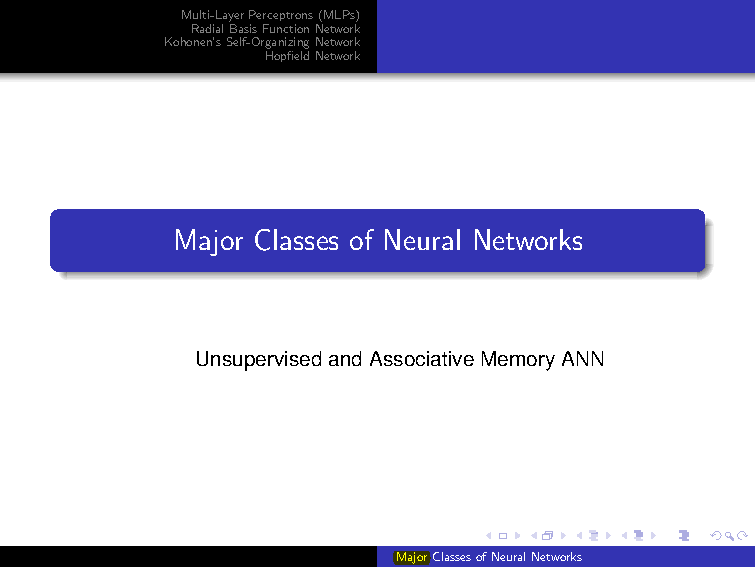
\includepdf[page=29]{slides}
There are many ways we can tweak our network.

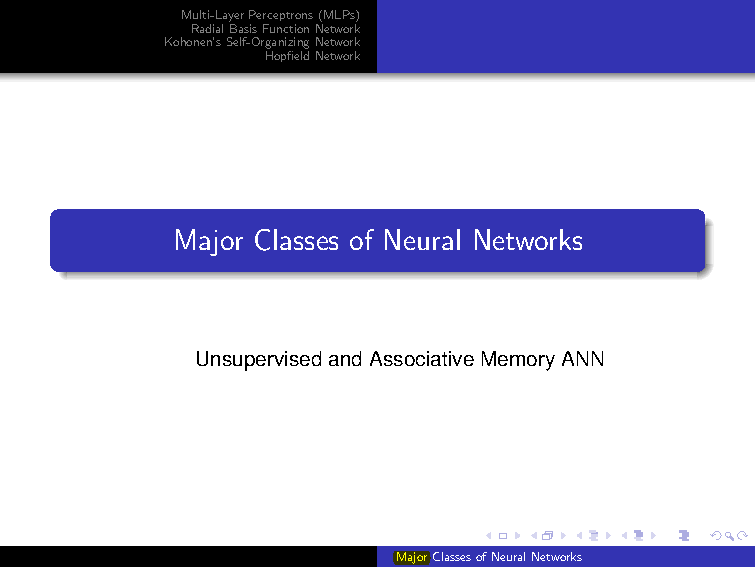
\includepdf[page=30-69]{slides}






\end{document}
